\documentclass{article}
\usepackage{amsmath}
\usepackage{amssymb}
\usepackage{mathtools}
\usepackage{graphicx}
\usepackage{enumitem}
\usepackage[margin=1in]{geometry}
\usepackage{titling}
\usepackage{xcolor}
\usepackage{bm}

\renewcommand{\vec}[1]{\mathbf{#1}}
\DeclareMathOperator{\Var}{Var}
\newcommand*\eval[3]{\left[#1\right]_{#2}^{#3}}
\newcommand{\mat}[1]{\mathbf{#1}}
\DeclareMathOperator*{\argmax}{arg\,max}
\DeclareMathOperator*{\argmin}{arg\,min}

\setlength{\droptitle}{-7em}   % This is your set screw

\begin{document}

\title{Machine Learning\\ Problem Set 1}
\author{Ozaner Hansha}
\date{September 29, 2020}
\maketitle

For the first 2 questions, consider a training dataset $\mathcal D=\{(\vec x_i,y_i)\}^n_{i=1}$, where $\vec x_i\in\mathbb R^d$. We then fit the data using linear least squares, i.e. finding the $\vec w$ that minimizes $\|\vec y-\mat X\vec w\|^2$ which nets us an optimal parameter vector $\vec w^*$ for use in the model:
$$y=\vec w^*\cdot\vec x$$

\textit{Note that each $\vec x_i$ in the data set has its first component equal to 1 (bias). Also note that $\vec w^*$ in this case (linear least squares) is given by $\mat X^+\vec y$.}

\subsection*{Question 1}
\noindent\textbf{Problem:} Consider a new dataset $\mathcal D'=\{(\vec x_i,y_i')\}^n_{i=1}$, where $y_i'=ay_i+b$ for some constants $a,b$. Fitting this data using linear least squares, we arrive at a new parameter vector $\vec w'$.

Can $\vec w'$ be computed directly from $\vec w^*$ and the constants $a,b$ without looking at the dataset? That is to say, can we express $\vec w'$ solely in terms of $\vec w^*, a,$ and $b$? If yes, how? If no, why not?
\bigskip

\noindent\textbf{Solution:} No, $\vec w'$ cannot be expressed without reference to the dataset. To see this, first note that the action on the labels of the dataset $\vec y$ is equivalent to the following:
\begin{align*}
    \vec y'=a\vec y+b\vec 1\tag{$\vec 1$ is a vector of 1s}
\end{align*}

Plugging this into the formula for $\vec w'$:
\begin{align*}
    w'&=\mat X^+\vec y'\tag{sol. to linear least squares}\\
    &=\mat X^+(a\vec y+b\vec 1)\tag{def. of $\vec y'$}\\
    &=a\mat X^+\vec y+b\mat X^+\vec 1\\
    &=a\vec w^*+b\mat X^+\vec 1\tag{def. of $\vec w^*$}
\end{align*}

We are left with the above sum and while we can express the first term referencing only $\vec w^*$ and $a$, the second term must make reference to $\mat X$. This reference is unavoidable as it is impossible to recover $\mat X$ from just $\vec w^*$.

And so, we cannot express $\vec w'$ without reference to the dataset. That said, as the first term shows, we could if there was no constant term $b$ added to each $y_i$.
\smallskip
\newpage

\subsection*{Question 2}
\noindent\textbf{Problem:} Consider a new dataset $\tilde{\mathcal D}=\{(\tilde{\vec x}_i,y_i)\}^n_{i=1}$, where $\tilde{x}_{ij}=c_j x_{ij}$ for some $d$ dimensional constant vector $\vec c$. Fitting this data using linear least squares, we arrive at a new parameter vector $\tilde{\vec w}$.

Can $\tilde{\vec w}$ be computed directly from $\vec w^*$ and $\vec c$ without looking at the dataset? That is to say, can we express $\tilde{\vec w}$ solely in terms of $\vec w^*$ and $\vec c$? If yes, how? If no, why not?
\bigskip

\noindent\textbf{Solution:} We can indeed express $\vec w'$ without reference to the dataset. First note that the action on the features of the dataset $\mat X$ is equivalent to the following product:
\begin{align*}
    \tilde{\mat{X}}&=\mat X\operatorname{diag}(c_1,\cdots,c_d)\\
    &=\mat{XC}\tag{let $C=\operatorname{diag}(c_1,\cdots,c_d)$}
\end{align*}

And so we have the following chain of equalities:
\begin{align*}
    \tilde{\vec w}&=\tilde{\mat{X}}^+\vec y\tag{sol. to linear least squares}\\
    &=(\mat{X}\mat{C})^+\vec y\tag{def. of $\tilde{\mat{X}}$}\\
    &=\mat{C}^+\mat{X}^+\vec y\tag{see note$^1$}\\
    &=\mat{C}^+\vec w^*\tag{def. of $\vec w^*$}\\
    &=\mat{C}^{-1}\vec w^*\tag{diagonal matrix is invertible}\\
    &=\operatorname{diag}(1/c_1,\cdots,1/c_d)\vec w^*\tag{inverse of diagonal matrix}
\end{align*}

\textit{$^1$The property $(\mat A\mat B)^+=\mat B^+\mat A^+$ only holds for two matrices $\mat A$ and $\mat B$ if they are of full rank. In this case, $\mat C$ is clearly full rank since it's a diagonal matrix, and we assume that $\mat X$ is also full rank. This is a reasonable assumption as it is increasingly unlikely that the rows of a dataset do not span the full rank as the number of, supposedly i.i.d., samples increase.}
\bigskip

And so each element of the new parameter vector $\tilde{\vec w}$ is given by:
$$\tilde{w}_i=\frac{w^*_i}{c_i}$$

\subsection*{Question 3}
\noindent\textbf{Problem:} Given a dataset $\mathcal D=\{(\vec x_i,y_i)\}^n_{i=1}$ There is a closed form solution to the optimal MLE estimator of the following model:
$$y=\vec w\cdot\vec x+v$$

Where the noise $v\sim\mathcal N(0,\sigma^2)$ for some $\sigma^2$ that is constant for all recorded samples.
\bigskip

Is there a closed form solution to the optimal MLE estimator of that same model but where the variance of the noise for each sample $\vec x_i$ is different? The variances are given by $\boldsymbol{\sigma^2}=(\sigma_1^2,\cdots,\sigma^2_n)$.
\bigskip

\noindent\textbf{Solution:} There is a closed form solution, and its derivation is similar to that of the homoscedastic error model. Before we produce the closed form solution, we define the following matrix $\mat C$:
$$\mat C=\operatorname{diag}(1/\sigma^2_1,\cdots,1/\sigma^2_n)$$

Also note that, rather than considering $v$ a normal RV with mean 0, we can consider each $Y_i\mid\vec x_i$ a RV with the following distribution:
$$Y_i\mid\vec x_i\sim\mathcal N(\vec w\cdot\vec x_i,\sigma^2_i)$$

Where each label $y_i$ is a realization of $Y_i\mid\vec x_i$.
\newpage

With these two facts in mind, we now find the paramater vector $\vec w^*$ that maximizes the likelihood of the observed data under the given linear model:
\begin{align*}
    \vec w^*&=\argmax_{\vec w}\,p(\vec y\mid\mat X;\vec w, \vec{\sigma^2})\tag{def. of optimal MLE parameter}\\
    &=\argmax_{\vec w}\prod_{i=1}^np(y_i\mid \vec x_i;\vec w,\sigma^2_i)\tag{$Y_i$ are independent RVs}\\
    &=\argmax_{\vec w}\log\prod_{i=1}^np(y_i\mid \vec x_i;\vec w,\sigma^2_i)\tag{$\log$ is monotone increasing}\\
    &=\argmax_{\vec w}\sum_{i=1}^n\log p(y_i\mid \vec x_i;\vec w,\sigma^2_i)\\
    &=\argmax_{\vec w}\sum_{i=1}^n\log\left(\frac{1}{\sigma^2_i\sqrt{2\pi}}e^{-\frac{(y_i-\vec w\cdot\vec x_i)}{2\sigma^2_i}}\right)\tag{$Y_i$ is a normal RV}\\
    &=\argmax_{\vec w}\sum_{i=1}^n\textcolor{red}{-\log(\sigma^2_i\sqrt{2\pi})}-\frac{(y_i-\vec w\cdot\vec x_i)^2}{2\sigma^2_i}\\
    &=\argmax_{\vec w}-\frac{1}{2}\sum_{i=1}^n\frac{(y_i-\vec w\cdot\vec x_i)^2}{\sigma^2_i}\tag{$\textcolor{red}{\text{red term}}$ independent of $\vec w$}\\
\end{align*}

Now to find $\vec w$ we can simply set the derivative of the expression we are trying to maximize equal to $\vec 0$, as quadratic polynomials have a single maximum:
\begin{align*}
    \vec 0&=\frac{\partial}{\partial\vec w}-\frac{1}{2}\sum_{i=1}^n\frac{(y_i-\vec w\cdot\vec x_i)^2}{\sigma^2_i}\\
    &=\frac{\partial}{\partial\vec w}\sum_{i=1}^n\frac{(y_i-\vec w\cdot\vec x_i)^2}{\sigma^2_i}\\
    &=\frac{\partial}{\partial\vec w}(\vec y-\mat X\vec w)^\top\mat C(\vec y-\mat X\vec w)\tag{$\mat C=\operatorname{diag}(1/\sigma^2_1,\cdots,1/\sigma^2_n)$}\\
    &=\frac{\partial}{\partial\vec w}(\vec y^\top-\vec w^\top\mat X^\top)\mat C(\vec y-\mat X\vec w)\\
    &=\frac{\partial}{\partial\vec w}\vec y^\top\mat C\vec y-\vec w^\top\mat X^\top\mat C\vec y-\vec y^\top\mat C\mat X\vec w+\vec w^\top\mat X^\top\mat C\mat X\vec w\\
    &=-\mat X^\top\mat C\vec y-(\vec y^\top\mat C\mat X)^\top+2\mat X^\top\mat C\mat X\vec w\\
    &=-\mat X^\top\mat C\vec y-\mat X^\top\mat C\vec y+2\mat X^\top\mat C\mat X\vec w\tag{$\mat C$ is symmetric}\\
    &=\mat X^\top\mat C\vec y-\mat X^\top\mat C\mat X\vec w\\
    \mat X^\top\mat C\mat X\vec w&=\mat X^\top\mat C\vec y\\
    \vec w&=(\mat X^\top\mat C\mat X)^{-1}\mat X^\top\mat C\vec y\tag{$\mat X$ is full rank}
\end{align*}

And so the MLE estimator is given by:
\begin{align*}
    y&=\vec w^*\cdot \vec x\\
    &=((\mat X^\top\mat C\mat X)^{-1}\mat X^\top\mat C\vec y)\cdot\vec x
\end{align*}

Note that this is identical to the weighted least squares (WLS) estimator with a weight matrix of $\mat C$.
\smallskip

% -- first attempt at an answer before I knew this was just weighted LSE --
% We can obtain a closed form solution for this model. First let us review the problem we are trying to solve, find the parameter vector $\vec w^*$ that maximizes the likelihood of seeing the labels $\vec y$ given the features $\mat X$ and their variances $\boldsymbol{\sigma^2}$:
% $$\argmax_{\vec w}\,p(\vec y\mid\mat X;\vec w,\boldsymbol{\sigma^2})$$

% Note that the model implies that each $y_i$ is a realization of a RV with the following distribution:
% $$y_i\sim\mathcal{N}(\vec w\cdot\vec x_i,\sigma_i^2)$$

% So, if we divide each $y_i$ by it's corresponding standard deviation $\sigma_i$ (i.e. standardize its variance) we arrive at a new vector of normal RVs $\vec z$ all with the same variance of 1:
% $$\frac{y_i}{\sigma_i}\sim\mathcal{N}\left(\frac{\vec w\cdot\vec x_i}{\sigma_i},1\right)$$

% Letting $y'_i=\frac{y_i}{\sigma_i}$ and $\vec x_i'=\frac{x_i}{\sigma_i}$ we have a familiar distribution:
% $$y'_i\sim\mathcal{N}(\vec w\cdot\vec x'_i,1)$$

% This transformation leads to the following model:
% \begin{align*}
%     y'&=\vec w\cdot \vec x'+v\tag{where $v\sim\mathcal{N}(0,1)$}
% \end{align*}

% The parameter vector $\vec w'$ that optimizes the above model is given by:
% $$\argmax_{\vec w}\,p(\vec y'\mid\mat X';\vec w,1)$$

% Recall that this is equivalent to the linear least squares solution given by:
% \begin{align*}
%     w'&=(\mat X')^+\vec y'\\
%     &=(\mat C\mat X)^+\mat C\vec y\tag{Let $\mat C=\operatorname{diag}(1/\sigma_1,\cdots,1/\sigma_n)$}\\
%     &=\mat X^+\mat C^+\mat C\vec y\\
%     &=\mat X^+\vec y\tag{$C^+=C^{-1}$}
% \end{align*}

% And so we have an optimal parameter vector $\vec w'$ that maximizes the likelihood of $\vec y'$. So we have:
% \begin{align*}
%     y'&=\vec w'\cdot\vec x'\\
%     &=
% \end{align*}
\newpage

\subsection*{Question 4}
\noindent\textbf{Problem:} After filling in the missing code for the gradient descent function, choose a polynomial model that best fits the population based off its RMSE on the validation set.
\smallskip

\noindent\textbf{Solution:} Based on the RMSE, the best polynomial model I found was the sixth order one. That is, the feature transformation $\bm{\phi}$ given by:
$$\bm{\phi}_6\left(\begin{bmatrix}
    x_{1} \\
    x_{2} \\
    \vdots \\
    x_{m}
  \end{bmatrix}\right)=\begin{bmatrix}
    1\\
    x_{1} \\
    x_{1}^2 \\
    \vdots \\
    x_{1}^6 \\
    x_{2} \\
    x_{2}^2 \\
    \vdots \\
    x_{m}^5\\
    x_{m}^6
  \end{bmatrix}$$
\bigskip

My methodology for determining this was to to compare the RMSE of increasingly large polynomial models until the error found a local minima. In this case it was at sixth degree features:
\begin{center}
    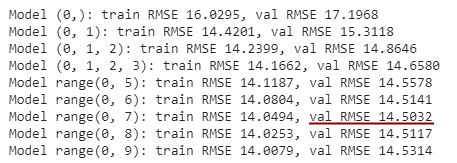
\includegraphics[scale=.95]{fig1.png}  
\end{center}

After this, I randomly removed certain degrees from the sixth order model and compared its RSME (e.g. instead of using the degrees $\{0,1,2,3,4,5,6\}$ I removed the fifth degree terms: $\{0,1,2,3,4,6\}$). However, all of these attempts resulted in a lower RSME and so I stuck with the complete sixth order model.

\subsection*{Question 5}
\noindent\textbf{Problem:} After filling in the missing code for the asymmetric loss function, choose a polynomial model that best fits the population based off its root mean asymmetric loss (RMAE), with $\alpha=.05$, on the validation set.
\bigskip

\noindent\textbf{Solution:} Based on the RMAE, the best polynomial model I found was the 29th order one. That is, the feature transformation $\bm{\phi}$ given by:
$$\bm{\phi}_{29}\left(\begin{bmatrix}
    x_{1} \\
    x_{2} \\
    \vdots \\
    x_{m}
  \end{bmatrix}\right)=\begin{bmatrix}
    1\\
    x_{1} \\
    x_{1}^2 \\
    \vdots \\
    x_{1}^6 \\
    x_{2} \\
    x_{2}^2 \\
    \vdots \\
    x_{m}^{28}\\
    x_{m}^{29}
  \end{bmatrix}$$
\bigskip

My methodology for determining this was the same as in question 4, to compare the RMAE of increasingly large polynomial models until the error found a local minima. In this case it was at 29th degree features:
\begin{center}
    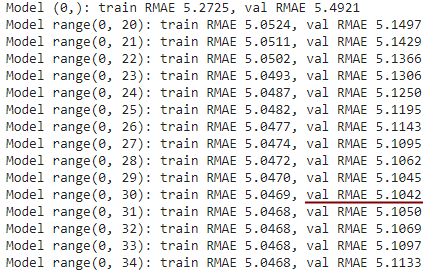
\includegraphics[scale=.95]{fig2.png}
\end{center}

\subsection*{Question 6}
\noindent\textbf{Problem:} Evaluate the two chosen models from question 4 and 5 on the test set with both the RMSE and the RMAE. Based on these results, discuss the relative merits of the two models for the data and task at hand. If you had to choose one, given the description of the prediction problem and the assumptions above, which one would you choose and why?
\bigskip

\noindent\textbf{Solution:} The results of running the 6th and 29th degree models on the test data are given below:
\begin{center}
    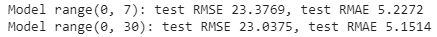
\includegraphics[scale=.95]{fig3.png}
\end{center}

As we can see, the 29th degree model does better in both RMSE \textit{and} RMAE. As a result, it seems reasonable to dub it the better model choice.

However performance isn't the only concern for such a model. In particular note that the 29th degree model is still very close to the 6th degree model in terms of performance. And that this slight increase in performance is contrasted by the huge increase in feature dimensionality:
\begin{align*}
    \operatorname{dim}(\bm{\phi}_6(\vec x))=14*6+1&=79\\
    \operatorname{dim}(\bm{\phi}_{29}(\vec x))=14*29+1&=378
\end{align*}

With greater dimensionality comes greater computational overhead. Although in this case, computing a prediction using the 29th degree model still isn't prohibitively expensive with reasonable hardware.

And so, it seems that, sans any other testing data, the 29th degree model is the better of the two models.

\end{document}